\chapter{Methodology}
\label{ch:methodology}

In data-assimilation terms, PI-CON learns a reconstruction operator that maps a sparse observation stream directly to the analysis field, replacing the iterative adjoint-and-solver loop of variational assimilation~\cite{Asch2016DA} with a single forward pass. For the DNS-free placement option, it also replaces the offline DNS trajectory of POD-based reduced-order models~\cite{Manohar2018PNAS} with a low-cost LES. This chapter follows one deployment instance: a long-horizon LES selects sensor positions via QR-pivoting on its POD basis; the physical flow supplies sensor values at those positions; PI-CON trains on the sensor time series and PDE residuals; and the trained operator reconstructs the continuous field on demand. In the controlled experiments below, a DNS field stands in for that real-world flow, sampled at the $K$ sensor positions for training and used as the offline evaluation reference; the full DNS field never enters the training objective. Figure~\ref{fig:architecture} shows the end-to-end signal flow.

% 圖原生 19.7 x 8.3 cm。出血 1.3x（19.5 cm）→ scale 0.99，字不縮反漲：
% 標題 11.9pt、描述 9.9pt，均過內文 12pt 的 80% = 9.6pt 門檻。
% 高度是硬約束：章首段落後僅剩約 10 cm，圖 8.2 + caption 2.2 = 10.4 cm 需實測不踢頁。
\begin{figure}[!htbp]
    \centering
    \makebox[\linewidth][c]{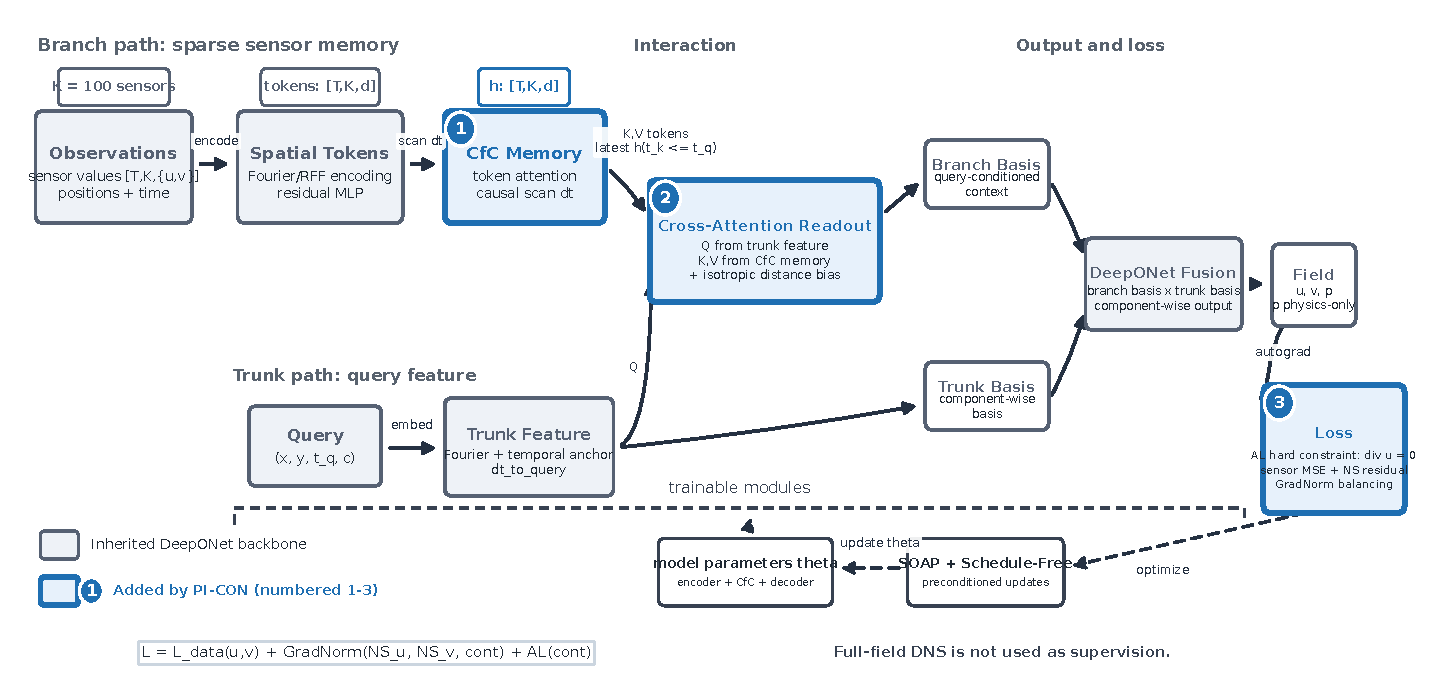
\includegraphics[width=1.3\linewidth]{figures/architecture/architecture.pdf}}
    \caption{PI-CON end-to-end signal flow. Grey boxes are the inherited DeepONet backbone; the three blue numbered boxes (1--3) are the additions in this work (1 CfC memory, 2 cross-attention readout, 3 the Augmented-Lagrangian continuity loss). Training uses sensor MSE and Navier--Stokes residuals only; no full-field DNS supervision.}
    \label{fig:architecture}
\end{figure}

\section{Engineering-Deployable Regime}
\label{sec:engineering_constraint}

Five conditions define the engineering deployment regime that every architectural and loss-design choice in this chapter must satisfy. They reflect the operational reality of in-situ flow reconstruction, where only sparse sensor measurements and the governing PDE are available rather than offline DNS post-processing.

\begin{enumerate}
    \item \textbf{Training supervision.} Only velocity components $(u,v)$ at sensor locations $\mathcal{S}$ supervise training. No DNS full-field signal enters, directly or through derived terms such as perceptual losses, spectral losses, VAE reconstructions, or latent priors.
    \item \textbf{Physics constraints.} The incompressible Navier--Stokes momentum and continuity residuals are enforced at random collocation points.
    \item \textbf{Data conditions.} DNS stands in for the experimentally inaccessible true flow in this controlled study, serving only to (a) extract sensor measurements at the LES-selected positions and (b) provide a reference field for offline a posteriori evaluation. \emph{The reference field never enters the training loss.}
    \item \textbf{Deployment assumption.} At deployment the model accesses only the same $K = 100$ fixed sensor positions and their time-stamped values; no DNS or full-field information is available.
    \item \textbf{Noise.} The main training runs use noise-free sensor measurements. Additive Gaussian noise robustness is a supporting engineering diagnostic; sensor-specific calibration errors lie outside the main objective.
\end{enumerate}

Figure~\ref{fig:pipeline} situates these conditions in the DNS-free deployment instance. Sensor placement is one of the sensing-configuration variables this work quantifies; here it takes the LES-derived, DNS-free form. The LES contributes sensor \emph{positions} only (a POD basis on which QR-pivoting selects the $K$ sites) and supplies no sensor values. The sensor \emph{values} are sampled at those positions from the DNS field that, in this controlled study, stands in for the experimentally inaccessible real-world flow. The label ``DNS-free'' therefore qualifies the placement step alone: siting the sensors needs no DNS, while the measurements read only $K$ point values and the full DNS field never enters training.

\begin{figure}[!htbp]
    \centering
    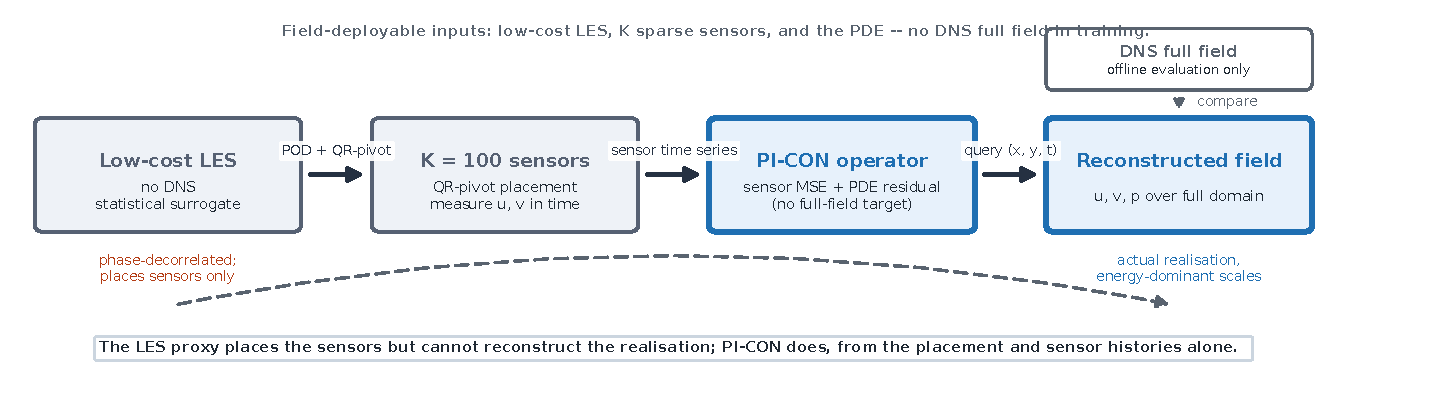
\includegraphics[width=\linewidth]{figures/architecture/pipeline.pdf}
    \caption{DNS-free deployment pipeline. The low-cost LES (green, top row) supplies only sensor \emph{positions} (POD + QR-pivot), not field values. Solid arrows: the deployable data path, where sensors read $u,v$ and PI-CON reconstructs a queryable $(u,v,p)$ field. Dashed: the full DNS field enters offline evaluation only, never training.}
    \label{fig:pipeline}
\end{figure}

\section{Modelling Assumptions}
\label{sec:assumptions}

The assumptions below are stated explicitly so that subsequent design choices and evaluation decisions remain amenable to local reasoning. The five supervision and deployment conditions of \S\ref{sec:engineering_constraint} are taken as given; the items below add further physical and numerical assumptions.

\begin{enumerate}
    \item \textbf{Governing equations.} The flow obeys the incompressible Navier--Stokes continuity and momentum equations (\S\ref{sec:problem_formulation}, equations~\eqref{eq:cont_main}--\eqref{eq:mom_main}). Compressibility, thermal effects, and non-Newtonian rheology are not modelled.
    \item \textbf{Geometry and boundary conditions.} The benchmark uses the periodic domain $\Omega = [0,1]^2$ with doubly periodic boundary conditions and no embedded obstacles. Non-periodic, wall-bounded, and obstacle-laden geometries are outside the present scope.
    \item \textbf{Known physical parameters.} The Reynolds number $Re$, kinematic viscosity $\nu = 1/Re$, forcing amplitude $A$, and forcing wavenumber $k_f$ are known a priori; parameter identification lies outside the inverse problem studied here.
    \item \textbf{Sensor placement and identity.} The sensor count $K$ and grid locations $\mathcal{S}$ are fixed before training and unchanged at inference, selected by QR-pivot on the POD basis (\S\ref{sec:sensor_placement}).
    \item \textbf{Channel availability.} Only the velocity components $(u, v)$ are measured at sensor positions. Vorticity $\omega$ serves as a diagnostic; pressure $p$ is a model-internal variable, not directly supervised.
    \item \textbf{Operator parameterization.} The reconstruction operator $\mathcal{G}_\theta$ is a single neural network returning $(u, v, p)$ at any query coordinate; no analytic decomposition or reduced-order basis is fixed outside the learnable parameters.
\end{enumerate}

\section{Governing Equations and Reconstruction Problem}
\label{sec:problem_formulation}

Consider an incompressible two-dimensional flow on the periodic domain $\Omega = [0,1]^2$ over the time interval $[0, T]$, governed by
\begin{subequations}
\label{eq:ns_main}
\begin{align}
    \nabla \cdot \mathbf{u} &= 0, \label{eq:cont_main}\\
    \frac{\partial \mathbf{u}}{\partial t} + (\mathbf{u}\cdot\nabla)\mathbf{u}
        &= -\nabla p + \nu\,\nabla^2 \mathbf{u} + \mathbf{f}, \label{eq:mom_main}
\end{align}
\end{subequations}
with $\mathbf{u}=(u,v)^T$, pressure $p$, and kinematic viscosity $\nu = 1/Re$. The Reynolds number used throughout is defined in \eqref{eq:re_def} as
\begin{equation}
    \label{eq:re_def}
    Re \;=\; \frac{U^* L^*}{\nu^*},
\end{equation}
where $L^* = 1$ m is the domain length scale, $U^* = 1$ m/s the reference velocity, and $\nu^*$ the kinematic viscosity. The main experiments use $Re = 10\,000$, giving $\nu^* = U^* L^* / Re = 10^{-4}$ m$^2$/s; the dimensionless form of \eqref{eq:ns_main} then has $\nu = 1/Re$. The Kolmogorov forcing is
\begin{equation}
    \label{eq:forcing}
    \mathbf{f}(\mathbf{x}) \;=\; \big(A\sin(2\pi k_f y),\; 0\big)^T,
\end{equation}
with $A = 0.1$, $k_f = 2$ in the main experiments at $Re=10\,000$.

\paragraph{Observation model.}
Measurements occupy $K$ fixed spatial locations $\mathcal{S} = \{\mathbf{x}_k\}_{k=1}^K$ at $N_t$ discrete time stamps $\{t_n\}_{n=1}^{N_t}$; each entry is $\mathbf{y}_{k,n} = (u(\mathbf{x}_k, t_n), v(\mathbf{x}_k, t_n))^T$. Per the engineering constraint of \S\ref{sec:engineering_constraint}, observed channels are restricted to $u$ and $v$; $\omega$ and $p$ are not measured.

\paragraph{Reconstruction target.}
The reconstruction operator is
\begin{equation}
    \label{eq:operator_def}
    \mathcal{G}_\theta : \;\big(\{\mathbf{y}_{k,n}\},\,\mathcal{S},\,\{t_n\}\big) \longmapsto (u, v, p)(\mathbf{x}, t)
\end{equation}
The operator in \eqref{eq:operator_def} is queriable at arbitrary $(\mathbf{x}, t) \in \Omega\times[0,T]$ and required to (i) match sensor observations on $\mathcal{S}\times\{t_n\}$ and (ii) satisfy the discrete residual of \eqref{eq:ns_main}. The parameters $\theta$ minimize the loss in \S\ref{sec:loss}.

\paragraph{Reconstruction target under an under-sampled snapshot.}
With $\mathbf{u}_t \in \mathbb{R}^N$ on the stored $256^2$ grid ($N = 65\,536$) and sensing operator $\mathbf{C}\in\{0,1\}^{K\times N}$, the snapshot equation $\mathbf{y}_t = \mathbf{C}\mathbf{u}_t$ is under-sampled: the compressed-sensing recovery threshold (\S\ref{sec:underdetermined}) sits roughly an order of magnitude above the $K=100$ budget, so exact pointwise recovery is not the goal. The achievable target is the energy-dominant low-wavenumber content: the architecture and physics constraints supply the structural prior that makes this band reconstructable, while the unresolved high-wavenumber modes lie beyond the sensor-count Nyquist scale $k_{\max}\approx\sqrt{K/\pi}$ (\S\ref{sec:underdetermined}).

\section{QR-pivot Sensor Placement}
\label{sec:sensor_placement}

Because $K \ll N$, sensor placement governs the achievable reconstruction error. The QRCP-on-POD-basis strategy of Manohar et al.~\cite{Manohar2018PNAS, Drmac2016SISC} selects $K$ row indices that minimize the conditioning of the sensing operator composed with the leading POD basis.

\paragraph{Snapshot matrix.}
$M$ snapshots $\{\mathbf{u}_{t_m}\}_{m=1}^M$ drawn uniformly from a DNS trajectory stack column-wise into $\mathbf{X}\in\mathbb{R}^{N\times M}$. The exposition treats $u$ as a single channel; the experiments use both measured velocity components to assemble the sensing basis.

\paragraph{POD basis.}
A truncated SVD,
\begin{equation*}
    \mathbf{X} \;=\; \mathbf{U}\,\boldsymbol{\Sigma}\,\mathbf{V}^T,
\end{equation*}
yields the dominant left singular vectors $\mathbf{U}_r = [\mathbf{u}_1\,|\,\cdots\,|\,\mathbf{u}_r]\in\mathbb{R}^{N\times r}$.

\paragraph{QRCP pivot selection.}
QR with column pivoting on $\mathbf{U}_r^T\in\mathbb{R}^{r\times N}$,
\begin{equation*}
    \mathbf{U}_r^T \,\mathbf{P} \;=\; \mathbf{Q}\,\mathbf{R},
\end{equation*}
yields a permutation $\mathbf{P}$ whose first $K$ columns identify the sensor grid locations $\mathcal{S}$. QRCP greedily picks columns that maximize the leading volume; the worst-case condition number of $\mathbf{C}\mathbf{U}_r$ obeys
\begin{equation*}
    \kappa(\mathbf{C}\mathbf{U}_r) \;\le\; \sqrt{1 + 4^K (N - K)}\,\frac{\sigma_{\max}(\mathbf{R}_{1:K,1:K})}{\sigma_{\min}(\mathbf{R}_{1:K,1:K})}.
\end{equation*}
In practice $\kappa$ from QRCP is much smaller than from random placement~\cite{Drmac2016SISC, Manohar2018PNAS}.

\paragraph{Concrete configuration.}
The main configuration sets $r$ automatically by a $99\%$ cumulative-variance threshold ($r\approx 60$), with $K=100$ and $M = 201$ DNS frames over $T=5$. The snapshot window spans one eddy turnover, so selected positions track dynamically informative regions.

\section{PI-CON Architecture}
\label{sec:architecture}

The architecture extends the contribution stated at the end of \S\ref{sec:research_questions}: vanilla DeepONet~\cite{Lu2021NMI} targets dense forward problems, and three of its building blocks must be replaced before it can address (O1)--(O3) under sparse sensing. Table~\ref{tab:deeponet_gaps} summarises the mapping; each gap is closed by one of the sub-networks introduced below.

\begin{table}[!htbp]
    \centering
    \caption{Three structural gaps of vanilla DeepONet under sparse-sensor reconstruction and the components introduced in this thesis to close them. All three additions build the reconstructor (O1); the right-hand column reports the role each plays.}
    \label{tab:deeponet_gaps}
    \small
    \setlength{\tabcolsep}{4pt}
    \begin{tabularx}{\textwidth}{>{\raggedright\arraybackslash}p{4.0cm}>{\raggedright\arraybackslash}p{4.4cm}>{\raggedright\arraybackslash}X}
    \toprule
    \textbf{Vanilla DeepONet gap} & \textbf{Addition in PI-CON} & \textbf{Role in the reconstructor (O1)} \\
    \midrule
    Branch ingests a fixed-grid snapshot; cannot handle an irregularly clocked sensor time signal. & Closed-form continuous-time (CfC) branch~\cite{Hasani2022CfC} (\S\ref{subsec:cfc_encoder}). & Reads the irregularly-clocked sensor time signal. \\
    Inner product is global; no spatial prior linking a query $(\mathbf{x},t)$ to the nearest sensors. & Cross-attention with isotropic distance bias~\cite{Vaswani2017Attention} (\S\ref{subsec:cross_attn}). & Sparse-to-dense field readout at any query. \\
    PDE residual is a soft penalty; continuity slips under sensor MSE alone. & Augmented-Lagrangian-style adaptive penalty on $\nabla\!\cdot\!\mathbf{u}$ (\S\ref{subsec:al_cont}). & Near-incompressible output field. \\
    \bottomrule
    \end{tabularx}
\end{table}

PI-CON comprises three sub-networks: (i) a sensor branch (spatial encoder, then a temporal CfC encoder, \S\ref{subsec:spatial_encoder}--\S\ref{subsec:cfc_encoder}); (ii) a trunk path (query encoder, \S\ref{subsec:trunk_path}); and (iii) a decoder (cross-attention, then DeepONet fusion, \S\ref{subsec:cross_attn}--\S\ref{subsec:operator_fusion}). The remaining components (learnable Fourier embedding~\cite{tancik2020fourierfeaturesletnetworks}, residual MLP encoder, and GradNorm auto-balancing~\cite{Chen2018ICML}) are standard and are introduced briefly where they appear.

\subsection{Sensor Branch: Spatial Set Encoder}
\label{subsec:spatial_encoder}

\paragraph{Motivation.}
The spatial set encoder converts the $K$ simultaneous point measurements into per-sensor feature vectors that retain each sensor's location, so the decoder can later weight each sensor by its proximity to a query point: the discrete analogue of attaching a basis function to every measurement station.

\paragraph{Inputs.}
At a single time stamp, sensor observations are $\mathbf{s} \in \mathbb{R}^{K\times 2}$ (already normalized) at locations $\{\mathbf{x}_k\}_{k=1}^K \in \Omega$.

\paragraph{Position encoding (Learnable Fourier embedding).}
The periodic domain calls for a learnable Fourier embedding. Each sensor location $\mathbf{x}_k = (x, y)$ is first periodicized as
\begin{equation*}
    \mathbf{e}(\mathbf{x}_k) \;=\; \big[\sin\!\tfrac{2\pi x}{L},\,\cos\!\tfrac{2\pi x}{L},\,\sin\!\tfrac{2\pi y}{L},\,\cos\!\tfrac{2\pi y}{L}\big]^T \;\in\;\mathbb{R}^4,
\end{equation*}
then linearly projected into the Fourier feature space:
\begin{equation}
    \label{eq:learnable_fourier}
    \gamma(\mathbf{x}_k) \;=\; \big[\cos(\mathbf{W}\,\mathbf{e}(\mathbf{x}_k)),\;\sin(\mathbf{W}\,\mathbf{e}(\mathbf{x}_k))\big]^T \;\in\;\mathbb{R}^{d_{\text{emb}}},
\end{equation}
where $\mathbf{W}\in\mathbb{R}^{(d_{\text{emb}}/2)\times 4}$ is initialized with $\mathcal{N}(0, \sigma^2)$ entries ($\sigma=2.0$) and learned jointly with the rest of the network ($d_{\text{emb}} = 128$). The trainable projection in \eqref{eq:learnable_fourier} adapts the frequency mixture and mitigates spectral bias~\cite{Rahaman2019Spectral}, unlike fixed-$\sigma$ Fourier features~\cite{tancik2020fourierfeaturesletnetworks}.

\paragraph{Token MLP and residual encoding.}
Concatenating position encoding and sensor measurement gives
\begin{equation*}
    \mathbf{f}_k \;=\; [\gamma(\mathbf{x}_k);\,\mathbf{s}_k] \;\in\;\mathbb{R}^{d_{\text{emb}}+2},
\end{equation*}
projected to width $d_{\text{model}} = 256$ by
\begin{equation*}
    \mathbf{e}_k^{(0)} \;=\; \mathrm{Linear}\!\big(\mathrm{SiLU}(\mathrm{Linear}(\mathrm{LayerNorm}(\mathbf{f}_k)))\big).
\end{equation*}
The token then passes through $L_s = 1$ residual MLP block:
\begin{equation}
    \label{eq:residual_block}
    \mathbf{e}_k^{(\ell)} \;=\; \mathbf{e}_k^{(\ell-1)} + \mathrm{MLP}\!\big(\mathrm{LayerNorm}(\mathbf{e}_k^{(\ell-1)})\big),\quad \ell=1,\ldots,L_s.
\end{equation}
The residual update in \eqref{eq:residual_block} is followed by an output projection (LayerNorm $\to$ Linear$_{d\to 2d}$ $\to$ SiLU $\to$ Linear$_{2d\to d}$) that yields the spatial token $\mathbf{z}_k \in \mathbb{R}^{d_{\text{model}}}$.

\paragraph{Design rationale.}
Tokens stay per-sensor rather than pooled, because the downstream cross-attention (\S\ref{subsec:cross_attn}) requires a per-query attention distribution over individual sensors: unrecoverable once pooled.

\subsection{Token Self-Attention}
\label{subsec:token_attn}

Neighbouring sensors sample correlated flow structures (a single vortex may straddle several stations), so each sensor's representation is sharpened by letting it attend to the others before the temporal branch evolves it. Before each CfC scan, sensor tokens pass through a token self-attention block~\cite{Vaswani2017Attention} (multi-head, $h=4$, $L_a=2$ layers):
\begin{equation}
    \label{eq:self_attn}
    \hat{\mathbf{Z}} \;=\; \mathbf{Z} + \mathrm{MultiheadAttn}(\mathrm{LayerNorm}(\mathbf{Z})),
    \quad \mathbf{Z}' \;=\; \hat{\mathbf{Z}} + \mathrm{FFN}(\mathrm{LayerNorm}(\hat{\mathbf{Z}})),
\end{equation}
with $\mathbf{Z} = [\mathbf{z}_1\,|\,\cdots\,|\,\mathbf{z}_K]^T \in\mathbb{R}^{K\times d_{\text{model}}}$ and FFN realised as Linear$_{d\to 2d}$ $\to$ SiLU $\to$ Linear$_{2d\to d}$. The update in \eqref{eq:self_attn} lets sensors exchange spatial information (e.g.\ upstream--downstream) while preserving the token identity required by the downstream causal cross-attention.

\subsection{Closing the Time-Signal Gap: CfC Continuous-Time Branch}
\label{subsec:cfc_encoder}

\paragraph{Motivation.}
The CfC branch compresses each sensor's time history into a compact state that tracks recent dynamics while tolerating irregular sampling intervals. Sensor time series $\mathbf{s}_k(t_n)$, $n=1,\ldots,N_t$, arrive on irregular clocks: packets drop, groups report on different cadences, and inference must accept whatever timestamps arrive. Discrete RNNs (GRU, LSTM) cannot absorb such irregular sampling; Neural ODE~\cite{Chen2018NODE} offers a continuous-time view at the cost of an ODE solver per step. CfC~\cite{Hasani2022CfC} provides a closed-form solution to LTC dynamics~\cite{Hasani2021LTC} at per-step cost comparable to a discrete RNN, and is therefore adopted here.

This choice also keeps training tractable on the stiff high-$Re$ case: stabilized MLP-based PINNs reach this regime by splitting the time domain into sequential windows and fitting one network per window (PirateNet~\cite{Wang2024JMLR} uses ten intervals, each initialized from the previous window's solution, and the second-order-optimized variant~\cite{wang2025gradientalignmentpinns} relies on time-marching and curriculum training), so their cost scales with the number of windows.

The CfC branch instead encodes the whole sensor time series in a single continuous-time pass, with a closed-form update that its authors report to train and run at least two orders of magnitude faster than ODE-based continuous-time models~\cite{Hasani2022CfC}; the liquid-network family it belongs to is also compact and noise-robust~\cite{Lechner2020NCP}. A CfC encoder is therefore preferred over a vanilla DeepONet branch or an MLP-PINN backbone for the sensor stream.

\paragraph{CfC cell.}
With cell input $\mathbf{c}_t \in \mathbb{R}^{d_{\text{in}}}$, hidden state $\mathbf{h}_t \in \mathbb{R}^{d_{\text{model}}}$, and time gap $\Delta t = t_n - t_{n-1}$, the CfC update is
\begin{subequations}
\label{eq:cfc}
\begin{align}
    f_1(\mathbf{c},\mathbf{h}) &= \tanh(\mathbf{W}_1[\mathbf{c};\mathbf{h}] + \mathbf{b}_1),\\
    f_2(\mathbf{c},\mathbf{h}) &= \tanh(\mathbf{W}_2[\mathbf{c};\mathbf{h}] + \mathbf{b}_2),\\
    \boldsymbol{\sigma}(\mathbf{c},\mathbf{h};\Delta t) &= \mathrm{sigmoid}\!\big(-\boldsymbol{\tau}_a\,\Delta t + \mathbf{t}_b([\mathbf{c};\mathbf{h}])\big),\\
    \mathbf{h}_{t+\Delta t} &= \boldsymbol{\sigma} \odot f_1 + (1-\boldsymbol{\sigma}) \odot f_2,
\end{align}
\end{subequations}
where $\mathbf{c}$ denotes the cell input (distinct from the spatial coordinate $\mathbf{x}$ used elsewhere) and $\mathbf{h}$ the recurrent hidden state. In the CfC update \eqref{eq:cfc}, $\boldsymbol{\sigma}$ blends a fast-response candidate state $f_1$ with a slow-relaxation candidate $f_2$. Because the time gap $\Delta t$ enters $\boldsymbol{\sigma}$ directly, a longer silence between sensor samples shifts the blend toward the relaxed state; this is how the cell absorbs irregular sampling instead of assuming a fixed clock. The element-wise time constants $\boldsymbol{\tau}_a = \exp(\boldsymbol{\tau}_a^{(\theta)})$ come from a learnable log-space parameter $\boldsymbol{\tau}_a^{(\theta)}\in\mathbb{R}^{d_{\text{model}}}$. It is initialized as $\mathrm{linspace}(\log\tau_{\min}, \log\tau_{\max}, d_{\text{model}})$ with $[\log\tau_{\min}, \log\tau_{\max}] = [-1, 1]$, so that $\tau \in [e^{-1}, e^{1}] \approx [0.37, 2.72]$; the exponential parametrization enforces positivity. The term $\mathbf{t}_b(\cdot) = \mathbf{W}_t[\mathbf{c};\mathbf{h}] + \mathbf{b}_t$ is a learnable input-dependent affine time shift.

\paragraph{Multi-layer multi-time scan.}
Let $L_t$ denote the number of CfC layers ($L_t = 1$ in the main experiment). Each layer performs (i) token self-attention vectorized over time, (ii) addition of a Reynolds-number bias $\mathbf{r}_e = \mathrm{Linear}(Re_{\text{norm}}) \in \mathbb{R}^{d_{\text{model}}}$ that lets the network adapt its time scales across $Re$, and (iii) a CfC forward scan. The CfC cell input at sensor $k$, time index $n$ is $\mathbf{c}_{k,n} = \mathbf{z}'_k + \mathbf{r}_e \in \mathbb{R}^{d_{\text{model}}}$ ($d_{\text{in}} = d_{\text{model}}$), the self-attention-refined spatial token tiled across $N_t$ time steps and shifted by the $Re$ bias:
\begin{equation*}
    \mathbf{h}_{k,n} \;=\; \mathrm{CfCCell}(\mathbf{c}_{k,n},\,\mathbf{h}_{k,n-1};\,\Delta t_n),
    \quad n=1,\ldots,N_t,\;k=1,\ldots,K,
\end{equation*}
with $\Delta t_n = t_n - t_{n-1}$. The output is the branch token-state tensor $\mathbf{H}\in\mathbb{R}^{N_t\times K\times d_{\text{model}}}$.

\paragraph{Bidirectional option (smoothing mode).}
An optional backward scan from $t_{N_t}$ to $t_1$ produces $\mathbf{h}^{(B)}_{k,n}$, added to the forward state $\mathbf{h}^{(F)}_{k,n}$. This mode applies to offline batch reconstruction (smoothing); deployment-oriented filtering uses the forward scan alone.

\subsection{Trunk Path: Query Encoding}
\label{subsec:trunk_path}

\paragraph{Query input.}
A query is $(x, y, t, c)$ with $c\in\{0, 1, 2\}$ indexing the output channel ($0\!=\!u$, $1\!=\!v$, $2\!=\!p$).

\paragraph{Spatial encoding.}
The Learnable Fourier embedding of the sensor branch (separate but identically structured weights) yields $\gamma(\mathbf{x}_q) \in \mathbb{R}^{d_{\text{emb}}}$.

\paragraph{Temporal encoding.}
The temporal feature combines an absolute phase anchor with a causal time gap. The phase anchor
\begin{equation*}
    \boldsymbol{\phi}(t) \;=\; \big[\sin\!\tfrac{2\pi n t}{T_{\text{total}}},\,\cos\!\tfrac{2\pi n t}{T_{\text{total}}}\big]_{n=1}^{N_h}\;\in\;\mathbb{R}^{2N_h},
\end{equation*}
with $N_h = 2$ and $T_{\text{total}} = 5$, supplies an absolute time reference independent of any relative offset. Given the latest sensor timestamp $t_{n^*(q)} \le t_q$, the causal time gap $\Delta t_q = t_q - t_{n^*(q)}$ projects to dimension $d_t = 16$ via $\mathbf{e}_t = \mathrm{Linear}(\Delta t_q)$.

\paragraph{Channel embedding.}
$\mathbf{e}_c = \mathrm{Embedding}(c) \in \mathbb{R}^8$ for $c\in\{0,1,2\}$.

\paragraph{Trunk feature.}
The concatenated input feeds a trunk MLP:
\begin{equation*}
    \mathbf{q}_{\text{trunk}} \;=\; \mathrm{TrunkMLP}([\gamma(\mathbf{x}_q);\,\boldsymbol{\phi}(t);\,\mathbf{e}_t;\,\mathbf{e}_c]) \;\in\;\mathbb{R}^{d_{\text{hidden}}},
\end{equation*}
an initial SiLU projection followed by $L_q = 1$ residual MLP blocks.

\subsection{Closing the Sparse-to-Dense Gap: Cross-Attention with Isotropic Distance Bias}
\label{subsec:cross_attn}

For each reconstruction point $(\mathbf{x}, t)$, the cross-attention readout learns how strongly every one of the $K=100$ sensors relates to that query. This turns query--sensor distance into a relevance weight, so the field value is built from location-specific sensor evidence rather than from a pooled comparison against the whole sensor set. This is the sparse-to-dense fusion required by the engineering setting: a continuous query must aggregate information from $K=100$ irregularly placed sensor tokens, with weights adapted to spatial proximity and physical similarity. Originating in the Transformer~\cite{Vaswani2017Attention} and extended by Perceiver~\cite{Jaegle2021Perceiver} to variable-size inputs, cross-attention natively handles irregular sensor sets. Two modifications adapt it to fluid reconstruction: an isotropic relative-position bias and a causal lookup over sensor time.

\paragraph{Causal lookup.}
Given query time $t_q$ and the strictly increasing sensor clock $\{t_n\}_{n=1}^{N_t}$, binary search returns the most recent timestamp not exceeding $t_q$:
\begin{equation}
    \label{eq:searchsorted}
    n^*(q) \;=\; \mathrm{clamp}\!\big(\mathrm{searchsorted}(\{t_n\},\,t_q,\,\mathrm{right=True}) - 1,\;0,\;N_t-1\big),
\end{equation}
the decoder then reads $\mathbf{H}_q = \mathbf{H}[n^*(q),\,:,\,:] \in \mathbb{R}^{K\times d_{\text{model}}}$. The lookup in \eqref{eq:searchsorted} enforces filtering causality: the query accesses sensor information only up to time $t_q$.

\paragraph{Isotropic relative-position bias.}
The cross-attention does \emph{not} use a directional relative position $(r_x, r_y)$. The isotropic distance kernel is a deliberate modelling simplification: although the Kolmogorov forcing $f_x = A\sin(2\pi k_f y)$ makes the flow statistically anisotropic, a directional bias would implicitly encode the non-uniform $x$-distribution of the QR-pivot sensors as a spurious directional attention term, whereas the isotropic norm $|\mathbf{r}|$ admits no such mechanism.

For query position $\mathbf{x}_q$ and sensor positions $\{\mathbf{x}_k\}$, the relative position $\mathbf{r}_{qk} = \mathbf{x}_q - \mathbf{x}_k$ folds onto the torus by
\begin{equation*}
    \mathbf{r}_{qk} \;\leftarrow\; \mathbf{r}_{qk} - L\cdot\mathrm{round}(\mathbf{r}_{qk}/L),
\end{equation*}
and a smooth norm follows:
\begin{equation}
    \label{eq:smooth_norm}
    r_{qk} \;=\; \sqrt{\Vert\mathbf{r}_{qk}\Vert_2^2 + \varepsilon},\quad \varepsilon = 10^{-8}.
\end{equation}
The $\varepsilon$ in \eqref{eq:smooth_norm} is required: when a collocation point coincides with a sensor ($\mathbf{r}_{qk}=\mathbf{0}$), the second-order autograd of $\Vert\mathbf{r}\Vert_2$, $(\Vert r\Vert^2 I - rr^T)/\Vert r\Vert^3$, evaluates to $0/0$ and yields a NaN inside the NS residual (observed on a non-periodic-domain test case where sensors and collocation points overlap with high probability). The smooth norm has a finite second derivative $\varepsilon^{-1/2}$ at $r = 0$, eliminating the NaN source.

The scalar distance maps to a scalar attention bias:
\begin{equation*}
    b_{qk} \;=\; \mathrm{MLP}_{\text{relpos}}(\mathrm{LayerNorm}(r_{qk})) \;\in\;\mathbb{R},
\end{equation*}
where $\mathrm{MLP}_{\text{relpos}}$ is LayerNorm $\to$ Linear$_{1\to d}$ $\to$ SiLU $\to$ Linear$_{d\to 1}$.

\paragraph{Cross-attention.}
Queries come from the trunk feature; keys and values from the branch token states. Let $\mathrm{TokenProj}:\mathbb{R}^{d_{\text{model}}}\!\to\!\mathbb{R}^{d_{\text{hidden}}}$ denote a single linear layer (with LayerNorm) applied per branch token before key/value projection:
\begin{align}
    \mathbf{Q}_q &= \mathbf{W}_Q\,\mathrm{LayerNorm}(\mathbf{q}_{\text{trunk}}),\\
    \mathbf{K}_k &= \mathbf{W}_K\,\mathrm{TokenProj}(\mathbf{H}_q[k]),\quad
    \mathbf{V}_k = \mathbf{W}_V\,\mathrm{TokenProj}(\mathbf{H}_q[k]).
\end{align}
The attention weights are
\begin{equation}
    \label{eq:attention}
    A_{qk} \;=\; \mathrm{softmax}_k\!\Big(\frac{\mathbf{Q}_q^T\mathbf{K}_k}{\sqrt{d_{\text{hidden}}}} + b_{qk}\Big),
\end{equation}
and the branch context is
\begin{equation*}
    \mathbf{c}_{\text{branch}}(q) \;=\; \sum_{k=1}^K A_{qk}\,\mathbf{V}_k + \mathrm{MLP}_{\text{ctx}}\!\Big(\sum_{k=1}^K A_{qk}\,\mathbf{V}_k\Big),
\end{equation*}
where $\mathrm{MLP}_{\text{ctx}}$ is a residual refinement of the attention output. Equation~\eqref{eq:attention} is the only place where the isotropic relative-position bias changes the attention logits.

\subsection{DeepONet-style Operator Fusion}
\label{subsec:operator_fusion}

\paragraph{Branch and trunk basis vectors.}
Each context vector projects onto a rank-$R$ basis ($R = 256$), sliced by channel $c$:
\begin{align}
    \boldsymbol{\Psi}^{\text{trunk}} &= \mathrm{Linear}_{d_{\text{hidden}}\to 3R}(\mathbf{q}_{\text{trunk}}) \in\mathbb{R}^{3\times R},\\
    \boldsymbol{\Psi}^{\text{branch}} &= \mathrm{Linear}_{d_{\text{hidden}}\to 3R}(\mathbf{c}_{\text{branch}}) \in\mathbb{R}^{3\times R}.
\end{align}
The channel-$c$ row yields $\boldsymbol{\psi}^{\text{trunk}}_c, \boldsymbol{\psi}^{\text{branch}}_c \in \mathbb{R}^R$.

\paragraph{Tensor-product fusion.}
The fusion mirrors a modal (POD-like) expansion: the trunk vector $\boldsymbol{\psi}^{\text{trunk}}_c$ supplies $R$ query-evaluated mode shapes, the branch vector $\boldsymbol{\psi}^{\text{branch}}_c$ the sensor-derived modal coefficients, and their inner product reconstructs the channel value the way $\sum_r a_r\phi_r(\mathbf{x})$ rebuilds a field from a POD basis. The DeepONet output is the element-wise inner product of the two basis vectors:
\begin{equation}
    \label{eq:fusion}
    \widetilde{u}_c(\mathbf{x}_q,t_q) \;=\; \tau_{\text{out}} \cdot \big(\boldsymbol{\psi}^{\text{trunk}}_c \odot \boldsymbol{\psi}^{\text{branch}}_c\big) \cdot \mathbf{1}
    \;=\; \tau_{\text{out}} \cdot \sum_{r=1}^R \psi^{\text{trunk}}_{c,r}\,\psi^{\text{branch}}_{c,r},
\end{equation}
with learnable scalar gain $\tau_{\text{out}} = \exp(\log\tau_{\text{out}}^{(\theta)})$ initialized at $1/\sqrt{R}$ (this DeepONet temperature is distinct from the CfC time-constant vector $\boldsymbol{\tau}_a$ of \S\ref{subsec:cfc_encoder}). A per-channel affine map then produces the prediction:
\begin{equation}
    \label{eq:output_head}
    u_c \;=\; \gamma_c\,\widetilde{u}_c + \beta_c,
\end{equation}
with learnable scalars $\gamma_c, \beta_c$ and $\gamma_c$ initialized to $g_{\text{out}} = 1$. The affine head in \eqref{eq:output_head} restores the channel-wise scale after the shared DeepONet basis expansion.

\paragraph{Inductive bias.}
Equation~\eqref{eq:fusion} expands the output as a sum of $R$ basis functions, each the product of a query-dependent trunk basis and a sensor-content-dependent branch basis. The factorization decouples spatial query from sensor encoding: once trained, the operator may be queried at any continuous coordinate $(\mathbf{x}, t)\in\Omega\times[0,T]$ without retraining or re-meshing, meeting the engineering need for on-demand reconstruction at arbitrary probe locations. The DeepONet universal-approximation theorem~\cite{Lu2021NMI} guarantees that any continuous operator can be approximated to arbitrary accuracy as $R \to \infty$; at finite $R$ the rank bounds effective capacity. The main experiment sets $R = d_{\text{model}} = 256$.

\section{Loss Function}
\label{sec:loss}

Per \S\ref{sec:engineering_constraint}, the training objective uses only sensor measurements at $\mathcal{S}\times\{t_n\}$ and the incompressible Navier--Stokes residual at random collocation points; no DNS full-field signal enters the loss. The objective is a weighted sum with weights dynamically adjusted by GradNorm auto-balancing~\cite{Chen2018ICML}:
\begin{equation}
    \label{eq:total_loss}
    \mathcal{L}(\theta) \;=\; w_{\text{data}}\,\mathcal{L}_{\text{data}}
                  + w_{\text{NS},u}\,\mathcal{L}_{\text{NS},u}
                  + w_{\text{NS},v}\,\mathcal{L}_{\text{NS},v}
                  + w_{\text{cont}}\,\mathcal{L}_{\text{cont}}
                  + \mathcal{L}_{\text{AL}},
\end{equation}
where $\mathcal{L}_{\text{AL}}$ is the Augmented-Lagrangian-style continuity penalty (\S\ref{subsec:al_cont}; $\mathcal{L}_{\text{AL}}=0$ when AL is disabled), added to the objective outside the GradNorm weighting. The four GradNorm-managed tasks in \eqref{eq:total_loss} are $\{\mathcal{L}_{\text{data}},\, \mathcal{L}_{\text{NS},u},\, \mathcal{L}_{\text{NS},v},\, \mathcal{L}_{\text{cont}}\}$; in the main configuration continuity enters both as this GradNorm-balanced soft term and through the adaptive AL penalty acting on the same residual.

\subsection{Sensor Data Loss with Initial-Condition Emphasis}

For $N$ randomly drawn observation triples $(\mathbf{x}_k, t_n, c)$ with $c \in \{0, 1\}$ ($u, v$):
\begin{equation}
    \label{eq:data_loss}
    \mathcal{L}_{\text{data}} \;=\; \frac{1}{N}\sum_{i=1}^{N} w_i\,\Big(\hat{u}_{c_i}(\mathbf{x}_i,t_i;\theta) - u^{\text{obs}}_{c_i}(\mathbf{x}_i,t_i)\Big)^2,
\end{equation}
where the data loss in \eqref{eq:data_loss} uses the IC weight
\begin{equation}
    w_i \;=\; \begin{cases} w_{\text{early}} & t_i \le t_{\text{early}},\\ 1 & t_i > t_{\text{early}}.\end{cases}
\end{equation}
The main experiment sets $t_{\text{early}} = 0.05$ and $w_{\text{early}} = 10$. The emphasis targets the initial-condition reconstruction window, which carries the highest per-step uncertainty in chaotic flow.

\subsection{NS Momentum Residuals}

Automatic differentiation of the network output yields the PDE residuals:
\begin{align}
    \label{eq:res_u}
    \mathcal{R}_u &= \frac{\partial u}{\partial t} + u\frac{\partial u}{\partial x} + v\frac{\partial u}{\partial y} + \frac{\partial p}{\partial x} - \nu\Big(\frac{\partial^2 u}{\partial x^2}+\frac{\partial^2 u}{\partial y^2}\Big) - f_x,\\
    \label{eq:res_v}
    \mathcal{R}_v &= \frac{\partial v}{\partial t} + u\frac{\partial v}{\partial x} + v\frac{\partial v}{\partial y} + \frac{\partial p}{\partial y} - \nu\Big(\frac{\partial^2 v}{\partial x^2}+\frac{\partial^2 v}{\partial y^2}\Big),
\end{align}
with $f_x = A\sin(2\pi k_f y)$. The two residuals in \eqref{eq:res_u}--\eqref{eq:res_v} share the same collocation batch, and the smooth norm \eqref{eq:smooth_norm} guarantees that second-order autograd produces no NaN at sensor-coincident points.

The momentum residual losses are
\begin{equation*}
    \mathcal{L}_{\text{NS},u} = \frac{1}{N_p}\sum_{j=1}^{N_p}\mathcal{R}_u^2(\mathbf{x}_j, t_j),\quad
    \mathcal{L}_{\text{NS},v} = \frac{1}{N_p}\sum_{j=1}^{N_p}\mathcal{R}_v^2(\mathbf{x}_j, t_j),
\end{equation*}
with $N_p = 1024$ random collocation points per step and $t_j \sim \mathcal{U}(0, t_{\max}(\text{step}))$, where $t_{\max}$ follows the time-marching curriculum (\S\ref{sec:training_protocol}).

\subsection{Continuity Residual}
\label{subsec:continuity}

\begin{equation}
    \label{eq:cont_res}
    \mathcal{R}_c \;=\; \frac{\partial u}{\partial x} + \frac{\partial v}{\partial y},\quad \mathcal{L}_{\text{cont}} = \frac{1}{N_p}\sum_{j=1}^{N_p}\mathcal{R}_c^2(\mathbf{x}_j,t_j).
\end{equation}

\subsection{Closing the Physics-Consistency Gap: Augmented Lagrangian on Continuity}
\label{subsec:al_cont}

The Augmented-Lagrangian-style (AL) term adds an adaptive penalty that progressively tightens the continuity constraint rather than merely discouraging its violation at a fixed weight. Incompressibility matters for engineering use: a field with large $\nabla\!\cdot\!\mathbf{u}$ is unphysical regardless of pointwise accuracy. GradNorm balances gradient magnitudes across the four tasks but imposes no floor on the continuity residual; an AL-style penalty~\cite{NocedalWright2006} augments the same mean-squared continuity residual $C \equiv \mathcal{L}_{\text{cont}}$ with a dual variable $\lambda$ that grows while the residual stays above zero:
\begin{equation}
    \label{eq:al_loss}
    \mathcal{L}_{\text{AL}} \;=\; \lambda\,C \;+\; \frac{\rho}{2}\,C^2,
\end{equation}
where $C = \mathcal{L}_{\text{cont}} = \frac{1}{N_p}\sum_{j=1}^{N_p}\mathcal{R}_c^2(\mathbf{x}_j, t_j)$ is the non-negative mean-squared divergence already entering the soft term, evaluated on the same collocation points, and $\rho > 0$ is the penalty strength. The penalty in \eqref{eq:al_loss} uses the squared residual rather than a signed mean, so it admits no sign cancellation: the constraint quantity is bounded below by zero. Every $\Delta_{\text{AL}} = 100$ steps the dual variable updates from an exponential moving average of $C$:
\begin{equation}
    \label{eq:al_update}
    \tilde{C}_{\text{ema}} \;\leftarrow\; (1-\beta)\,\tilde{C}_{\text{ema}} \;+\; \beta\,C,\qquad
    \lambda \;\leftarrow\; \mathrm{clip}\!\Big(\lambda + \rho\,\tilde{C}_{\text{ema}},\;0,\;\Lambda_{\max}\Big),
\end{equation}
with $\beta=0.5$ and clip ceiling $\Lambda_{\max}=10$. Because $C \ge 0$, the update in \eqref{eq:al_update} drives $\lambda$ monotonically upward, with $\Lambda_{\max}$ bounding it from above; the multiplier settles as the residual falls rather than by reaching that bound. The scheme thus acts as an accumulated-multiplier penalty schedule that steadily raises the effective continuity weight, rather than a textbook equality-constraint Lagrangian (whose multiplier would change sign). The lower clip at zero keeps $\lambda$ physically non-negative.

When AL is on, $\mathcal{L}_{\text{AL}}$ is added to the objective \eqref{eq:total_loss}, so GradNorm still manages the four-task weights while AL applies added pressure through $\lambda$. The penalty strength $\rho$ is a tuneable hyperparameter.

\subsection{GradNorm Auto-balancing}
\label{subsec:gradnorm}

The four loss terms differ markedly in scale across training, so static weighting cannot cope with the resulting dynamics. Equalizing the per-task gradient magnitudes automates the weight tuning a practitioner would otherwise perform by hand, preventing large momentum-residual gradients from swamping the much smaller continuity gradient (or the reverse). A custom GradNorm scheme adapted from~\cite{Chen2018ICML, Sener2018MOO} is used. Every $\Delta_g = 1\,000$ steps, per-task gradient norms are computed against a reference parameter $\theta_r$ (the trunk output linear-layer weight and bias); equalization-target weights are then derived, normalized against $w_{\text{data}}^{\text{target}}$ to suppress absolute scale drift, and EMA-smoothed:
\begin{align}
    G_i &= \Vert \nabla_{\theta_r} \mathcal{L}_i \Vert_2,
        \quad i\in\{\text{data},\,\text{NS-u},\,\text{NS-v},\,\text{cont}\},\\
    w_i^{\text{target}} &= \frac{\overline{G}}{G_i + 10^{-5}\overline{G}},
        \qquad \overline{G} = \tfrac{1}{4}\sum_i G_i,\\
    w_i^{\text{norm}} &= w_i^{\text{target}} / w_{\text{data}}^{\text{target}},\\
    w_i^{(\text{new})} &= m\,w_i^{(\text{old})} + (1-m)\,w_i^{\text{norm}},\quad m = 0.9,
\end{align}
where $w_i^{(\text{new})}$ may be clamped from below by a non-negative floor. In the main experiments dynamic balancing alone gave stability over $20\,000$ training steps.

\paragraph{Differences from the original GradNorm.}
Chen et al.~\cite{Chen2018ICML} use a relative training rate to compute target weights. The present variant directly equalizes gradient norms against a reference parameter, normalizes by $w_{\text{data}}^{\text{target}}$ to suppress absolute scale drift, and EMA-smooths to damp oscillations. Initial weights $[w_{\text{data}}, w_{\text{NS},u}, w_{\text{NS},v}, w_{\text{cont}}] = [1, 0.057, 0.057, 0.01]$ start the momentum terms at $5.7\%$ and continuity at $1\%$ of the data weight.

\section{Optimization Stack}
\label{sec:optimization}

The coupled sensor-MSE and PDE-residual objective is stiff and ill-conditioned: the second-derivative (Laplacian) physics terms and the data term curve differently, so a quasi-second-order optimizer that rescales the gradient by an approximate Hessian converges where plain first-order Adam stalls. The components below implement this idea.

\paragraph{SOAP optimizer.}
SOAP~\cite{Vyas2024SOAP}, a quasi-second-order method that approximates the Hessian via Shampoo-style factorization and applies Adam in the preconditioner eigenbasis, is adopted here following its use for second-order PINN optimization~\cite{wang2025gradientalignmentpinns}; it gives better stability than vanilla Adam in the multi-task PINN setting. Main settings: Adam-style betas $(0.9,0.999)$, frequent preconditioner updates, initial learning rate $10^{-3}$.

\paragraph{Schedule-Free wrapper.}
SOAP is wrapped in a Schedule-Free~\cite{ScheduleFree2024} layer that performs Polyak--Ruppert averaging in place of explicit learning-rate decay.

\paragraph{Learning-rate schedule.}
A staircase decay applies: linear warmup over $2\,000$ steps to $\text{lr} = 10^{-3}$, then multiplicative decay $\gamma_{\text{decay}} = 0.9$ every $2\,000$ steps. ($\gamma_{\text{decay}}$ avoids collision with the AL dual variable $\lambda$ of \S\ref{subsec:al_cont}.) Gradient clipping is enforced at $\Vert g\Vert_\infty \le 1.0$.

\section{Training Protocol}
\label{sec:training_protocol}

\paragraph{Time-marching curriculum.}
Following the causality principle of Wang 2022~\cite{wang2022respectingcausality}, collocation and query times are capped at
\begin{equation*}
    t_{\max}(s) \;=\; t_{\text{start}} + (T - t_{\text{start}})\cdot\min\!\Big(\frac{\max(0,\,s-s_w)}{\Delta s},\;1\Big),
\end{equation*}
with $t_{\text{start}}=0.5$, no fixed hold ($s_w = 0$), and a linear ramp of $\Delta s = 2\,000$ steps. The horizon expands from $t \le 0.5$ at the first step to the full $t \le T = 5$ by step $2\,000$, then stays at $T$, blocking early-time chaotic error from contaminating the global loss.

\paragraph{Sensor temporal trimming.}
While $t_{\max}(s) < T$, the sensor branch encoder reads only $t \le t_{\max}(s)$, keeping the CfC branch consistent with the query-side time-marching restriction.

\paragraph{Physics warmup / ramp.}
GradNorm balances physics weights dynamically; no additional warmup ramp is imposed. Random collocation drives the physics residuals throughout training.

\paragraph{Training loop.}
Algorithm~\ref{alg:training} summarizes the full procedure.

\begin{algorithm}[H]
\SetAlgoLined
\small
\caption{PI-CON training loop (filtering mode)}
\label{alg:training}
\KwIn{Sensor data $\mathbf{D}=\{\mathbf{y}_{k,n}\}$, positions $\mathcal{S}$, times $\{t_n\}$, iterations $S$.}
\KwOut{Trained parameters $\theta^*$.}
Initialize $\theta$; set $\mathbf{w}=[1, 0.057, 0.057, 0.01]$\;
\lIf{AL enabled}{set $\lambda \leftarrow 0$, $\tilde{C}_{\text{ema}} \leftarrow 0$}
\For{$s = 1$ \KwTo $S$}{
    Update curriculum $t_{\max}(s)$; trim sensors to $t \le t_{\max}(s)$\;
    $\mathbf{Z} \leftarrow \mathrm{SpatialSetEncoder}(\mathbf{D}, \mathcal{S})$\;
    $\mathbf{H} \leftarrow \mathrm{TemporalCfC}(\mathbf{Z}, \{t_n\})$\;
    Sample $N$ data triples (IC emphasis) and $N_p{=}1024$ collocation points\;
    Cross-attention with isotropic relpos, then DeepONet fusion $\to (u,v,p)$\;
    Compute $\mathcal{L}_{\text{data}}, \mathcal{L}_{\text{NS},u}, \mathcal{L}_{\text{NS},v}, \mathcal{L}_{\text{cont}}$\;
    \lIf{AL enabled}{compute $\mathcal{L}_{\text{AL}} = \lambda C + \frac{\rho}{2}C^2$ and add to total loss}
    \lIf{$s \bmod 1\,000 = 0$}{update $\mathbf{w}$ via GradNorm}
    $\theta \leftarrow \theta - \mathrm{SOAP{+}SF}(\nabla_\theta(\mathbf{w}\cdot\boldsymbol{\mathcal{L}}))$\;
    \lIf{AL enabled \textbf{and} $s \bmod 100 = 0$}{$\tilde{C}_{\text{ema}} \leftarrow (1{-}\beta)\tilde{C}_{\text{ema}} + \beta C$; $\lambda \leftarrow \mathrm{clip}(\lambda + \rho \tilde{C}_{\text{ema}}, 0, \Lambda_{\max})$}
}
\Return{$\theta^*$}
\end{algorithm}
